\chapter{Eletrônica}
\label{eletronica}

\section{MSP430} % (fold)
\label{sec:msp430}

É um microcontrolador RISC de 16 bits criado pela Texas Instrumets para aplicações de baixo consumo de energia.

% Colocar aqui sobre o que é o MSP430, sua função no projeto como foi utilizado


\subsection{MSPGCC} % (fold)
\label{sub:mspgcc}

É um porte do \textit{GNU C Compiler} (\textbf{GCC}) e do \textit{GNU Binutils} (\textbf{as}, \textbf{ld}) para o microcontrolador \textit{MSP430}. São providenciadas ferramentas para depuração e \textit{download} de binário (\textbf{GDB, JTAG} e \textbf{BSL}).


\section{Circuitos} % (fold)
\label{sec:circuito}

\subsection{Tacômetro} % (fold)
\label{sub:tac_metro}

\begin{figure}[h]
  \centering
	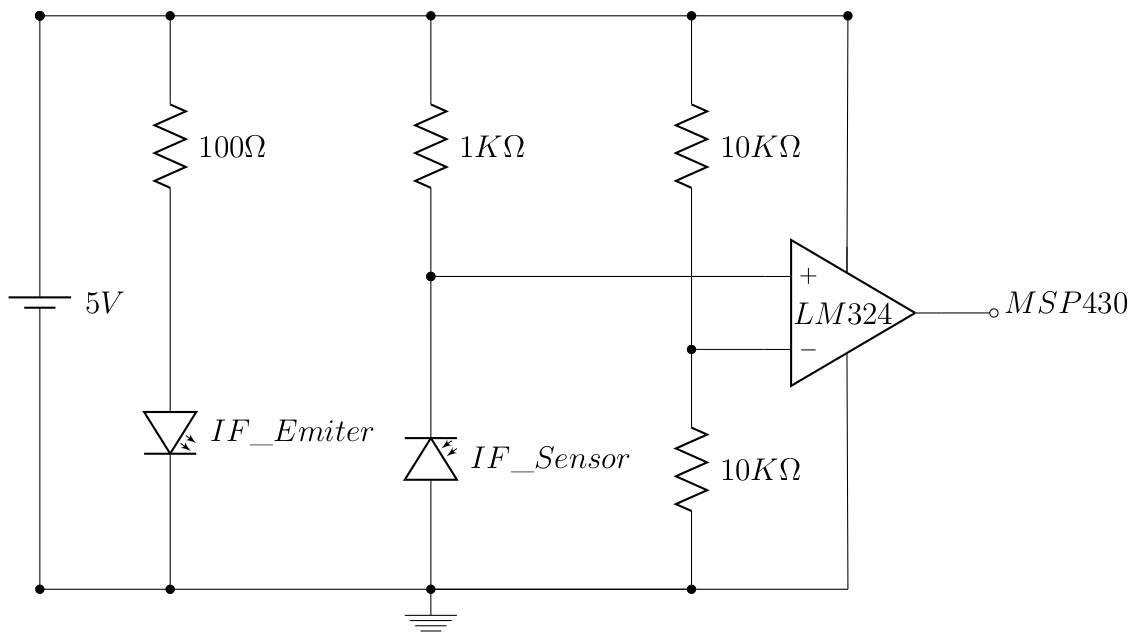
\includegraphics[width=0.8\textwidth]{figuras/tacometro}
  \caption{Circuito do Tacômetro}
  \label{fig:figuras_tacometro}
\end{figure}

% \begin{figure}[h]
% 	\centering
% 	\begin{circuitikz}[american,scale=0.7]

% 	\draw
% 	(2.5,0) node[short] (init) {}
% 	(10,-11) node[ground] (g) {}
% 	(18.1,-5.7) node[op amp,yscale=-1] (opamp){}
% 	(opamp.+) node[left] {}
% 	(17.9,-5.7) node[open]  {$LM324$}
% 	(opamp.-) node[left] {}
% 	(opamp.out) --  ++(1,0) node[ocirc,o-*] {~$MSP430$}
% 	(opamp.up) to [short] (18,-11) to (g)
% 	(opamp.down) ++ (0,.5) node[above] {} -- (opamp.down)
% 	;

% 	\draw
% 	(g) to [short] (2.5,-11) to [battery1,l_=$5V$,n=cap,*-*] ++(0,11)  to (init)
% 	(init)  to[short, *-*] (18,0) to (opamp.down)  ++(3,-3)
% 	(init)  to[short, *-*] (5,0) to [R,l^=$100\Omega$] ++(0,-5) to [empty led,l^=$IF\_Emiter$,-*] (5,-11) to (g)
% 	(init)  to[short, *-*] (10,0) to [R,l^=$1K\Omega$] ++(0,-5) to [short,n=in1,*-*] ++(0,0) 
% 	(g) to [pD,l^=$IF\_Sensor$,*-,mirror] ++(0,5) to (in1)
% 	(in1) to (opamp.+)
% 	(init)  to[short, *-*] (15,0) to [R,l^=$10K\Omega$] ++(0,-5)  to [short] ++(0,-1.40)to [short,n=in2,-*] ++(0,0) to [R,l^=$10K\Omega$,-*] (15,-11) to (g)
% 	(in2) to (opamp.-)
% 	;

% 	\end{circuitikz}
% 	\caption[Tacômetro]{Circuito do Tacômetro}
% 	\label{circ}
% \end{figure}

\subsection{Atuador do freio} % (fold)
\label{sub:atuador}

Será usado um servo motor para o controle do atuador do freio. Este servo motor é controlado por meio de uma onda PWM (\textit{Pulse Width Modulation}). Ondas PWM são usadas para controlar circuitos analógicos de forma digital, o que reduz o custo de produção e consumo do sistema. Por meio do uso de contadores de alta resolução, o \textit{duty cicle} de uma onda quadrada pode ser modulado para codificar certo valor de um sinal analógico. A tensão de controle é obtida com a constante mudança de pulsos que hora está na tensão máxima (ligado), hora está em 0 V (desligado). O tempo que este sinal fica na tensão máxima é chamado de \textit{duty cicle} de um sinal PWM (Figura \ref{fig:pwmcircuito}). Com uma repetida série de pulsos, a uma frequência satisfatória, é possível obter qualquer valor de tensão entre o máximo e mínimo valor do sinal digital.
Se um sinal PWM possui, por exemplo, 40\% de \textit{duty cicle} significa que o sinal digital está em seu valor máximo durante 40\% do seu período e está desligado durante 60\% do seu período. Caso a tensão de alimentação seja 9 V, a tensão que será medida na carga é de 40\% de 9 V, ou seja, 3,6 V.
%Atualizar figura
\begin{figure}[h]
  \centering
	% \includegraphics[width=0.8\textwidth]{pwmCircuito}
  \caption{Exemplo de sinal PWM com diferentes duty cicles.}
  \label{fig:pwmcircuito}
\end{figure}


Como dito anteriormente, o sinal PWM deve possuir uma frequência de variação entre os pulsos de forma que a carga “veja” uma tensão analógica constante. Suponha que um sinal PWM está em seu valor máximo durante 100 ms e depois muda para 0 V e fica neste estado por outros 100 ms. Se este ciclo se repetir 60 vezes por segundo, a tensão medida na saída será de 50\% da tensão máxima com frequência de 60 Hz. A esta frequência é dado o nome de frequência de modulação e depende do tipo sistema que será controlado.
Este método foi escolhido devido a sua grande imunidade a ruído, fácil controle da tensão de saída e redução do consumo total do sistema.

\subsection{Sensor Infravermelho} % (fold)
\label{sub:sensor_infra}

Sensores Infravermelhos são detectores que possuem uma fotocélula capaz de reagir à emissão de luz infravermelha. São muito utilizado em controles remotos, teclados, mouses sem fio, bem como, no isolamento de circuitos elétricos e sensores de posição. Todos os aparelhos de TV e DVD player possuem estes sensores para comandar alguma ação nestes aparelhos. O sinal é enviado por um LED emissor de luz infravermelha, é captado por um fototransistor e, por fim, os dados são processados. 
A aplicação destes sensores, juntos, é chamada de par ótico. Estes par ótico pode ser fabricado em diversos formatos, geralmente customizados para aplicações específicas. É possível encontrar o LED emissor e o fototransistor montados em um único encapsulamento para sensores de posição, com um sulco entre eles (Figura \ref{fig:fotoUni}), ou de forma separada funcionando como chaves óticas (Figura \ref{fig:fotoLED}), por exemplo.

\begin{figure}
        \centering
        \begin{subfigure}[b]{0.4\textwidth}
                % \includegraphics[width=0.8\textwidth]{pwmCircuito}
                \caption{LED e Fototransistor montados em um único encapsulamento}
                \label{fig:fotoUni}
        \end{subfigure}%
        ~
        \begin{subfigure}[b]{0.4\textwidth}
                % \includegraphics[width=0.8\textwidth]{pwmCircuito}
                \caption{Fototransistor separado do LED}
                \label{fig:fotoLED}
        \end{subfigure}
        \caption{Conjuntos de LED emissor e o fototransistor}
        \label{fig:LED}
\end{figure}